\documentclass[11pt,a4j,fleqn]{jarticle}
\usepackage{amsmath,amsthm,amssymb}
\usepackage[dvipdfmx]{graphicx}

\title{文書タイトル}
\author{大野 嵩侃}
\date{2014年6月7日}


\begin{document}

\maketitle

\section{はじめに}



\section{包絡線定理}

包絡線定理の解説を書く.

数式(番号なし)の例
\[
f(x, t) = t x - t^2
\]


数式(番号つき)の例
\begin{equation}
f(x, t)  = -(t - \frac{x}{2})^2 + \frac{x^2}{4} \label{eq:square}
\end{equation}

数式(番号つき)の例(高さが調整されたカッコ)
\begin{equation}
f(x, t) = -\left(t - \frac{x}{2}\right)^2 + \frac{x^2}{4} \label{eq:square-2}
\end{equation}



数式番号の引用の例:
平方完成の式\eqref{eq:square}より...

\begin{figure}
 \centering
 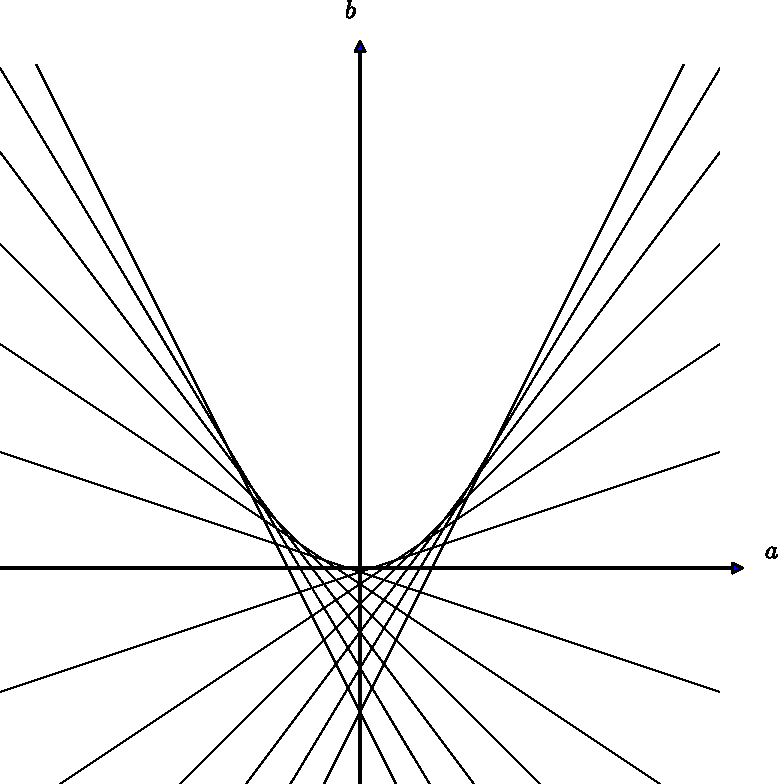
\includegraphics{envelope0.pdf}
 \caption{1つ目の図の表示}
 \label{fig:1}
\end{figure}

\begin{figure}
 \centering
 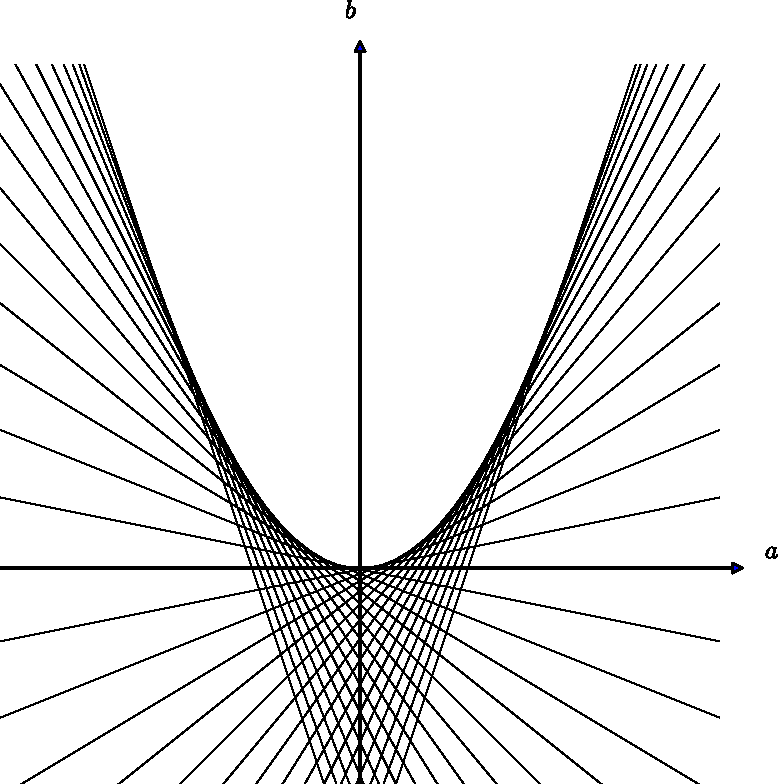
\includegraphics{envelope1.pdf}
 \caption{2つ目の図の表示}
 \label{fig:2}
\end{figure}



引用の例:尾山・安田\cite{OyamaYasuda11}.


\subsection{サブセクションのタイトル}

必要ならサブセクションを作る.



\section{Pythonプログラム}

自分のPythonプログラムの説明を書く.

コードの表示の例
\begin{quote}
\begin{verbatim}
from __future__ import division  # (p,q)区間をn-1等分するので小数が含まれる場合に対応させる
from numpy import linspace
from numpy import fabs
from mpl_toolkits.axes_grid.axislines import SubplotZero
import matplotlib.pyplot as plt
# ここから下に変数が入る


def f(x, a):
    return a*x-x**2  # 包絡線の式を入れる
p = -3  # xの最小値
q = 3  # xの最大値
n = 12  # 引く包絡線の数
a_min = -10  # 表示させるaの最小値
a_max = 10  # 表示させるaの最大値
y_min = -6  # 表示させるbの最小値(最大値はa軸とb軸の縮尺が1:1になるよう自動で決まる)
# アスペクト比を定めただけだと異常に縦長なグラフが出てくるのでylimを定めた
y_max = y_min+a_max-a_min  # これは変数ではない
plt.figtext(0.85, 0.35, '$a$')  # 直接位置を指定しているので、グラフの位置を変えるときにこれも変える
plt.figtext(0.5, 0.95, '$b$')
# ここより上に変数が入る
fig = plt.figure(1)
ax = SubplotZero(fig, 111)
fig.add_subplot(ax)
ax.axhline(linewidth=1.0, color="black")
ax.axvline(linewidth=1.0, color="black")
ax.set_xticks([])  # 空のlistを指定することでticksが入らない
ax.set_yticks([])
ax.set(aspect=1)
plt.figtext(0.85, 0.35, '$a$')  # 直接位置を指定している
plt.figtext(0.5, 0.95, '$b$')
for direction in ["xzero", "yzero"]:
    ax.axis[direction].set_axisline_style("-|>")
    ax.axis[direction].set_visible(True)
for direction in ["left", "right", "bottom", "top"]:
    ax.axis[direction].set_visible(False)
plt.ylim(ymin=y_min)  # この位置より前に置くとx方向が狭くなってしまった
plt.ylim(ymax=y_max)
a = linspace(a_min, a_max, (a_max-a_min) * 10)  # プロットする点の数はaが1増えるごとに10増えるようにした
for i in range(n):
    r = p+(q-p)*i/(n-1)  # n個の接線を引き2個は両端にあるので区間はn-1等分される
    b = f(r, a)
    ax.plot(a, b, 'k', linewidth=0.5, alpha=1)
# linewidth:線の太さ, alpha:濃さ(1以下), 黒色の線は'k'
plt.show()
# plt.savefig('envelopeX.png', bbox_inches='tight', pad_inches=0)
# plt.savefig('test2.pdf,bbox_inches='tight',pad_inches=0)
# それぞれ画像保存用,PDF保存用
\end{verbatim}
\end{quote}

\verb|\begin{verbatim}| ... \verb|\end{verbatim}| の中では改行は自動ではされない.
長すぎてページからはみ出す行は自分で適宜改行する.



\begin{thebibliography}{0}
\bibitem{OyamaYasuda11}
尾山大輔・安田洋祐「経済学で出る包絡線定理」『経済セミナー』2011年10・11月号.
\end{thebibliography}

\end{document}
